% !TEX root = ../../Beamer/02ForceVectors/02ForceVectors.tex

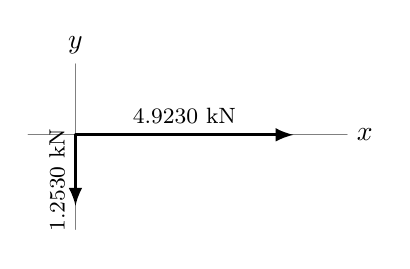
\begin{tikzpicture}[scale = 0.6, style={line cap = round}]
	
	\draw[gray](-1,0) -- (5.75,0) node[black, right] {$x$};
	\draw[gray] (0, -2) -- (0, 1.5) node[black, above] {$y$};
	\uncover<2->{
		\draw[very thick, -latex] (0, 0) -- node[above, sloped]{\footnotesize $4.9230$ kN} (4.613, 0);
	}
	\uncover<3->{
		\draw[very thick, latex-] (0, -1.5) -- node[above, xshift=-0.125cm, sloped]{\footnotesize $1.2530$ kN}  (0, 0);
	}

	%  \draw[<->] (2.5cm, 0mm) arc[start angle = 0, end angle = 33, radius = 2.5cm];
	%  \node [rectangle, right] at (2.4, 0.7) {\small $33\degree$};
	% \uncover<2->{
	%   \draw (0, -1.253) -- (4.613, -1.253) -- (4.613, 0);
	% }
	% \uncover<3->{
	%   \draw[very thick, saitRed, ->, >=stealth] (0, 0) -- node[above, sloped, very near end]{\footnotesize $\bm{\mathrm{ F }_{R}}$}(4.613, -1.253);
	%   \draw[<->] (2, 0)  arc[start angle = 0, end angle = -15.2, radius = 2cm] ;
	%   \node at (2.2, -0.3) {\footnotesize $\theta$};
	% }
\end{tikzpicture}
